\section{Clustering}

\subsection{Methods}
\todo[inline]{Describe each clustering method with important parameters that could influence the outcome}
\subsubsection{K-Means} \label{theory:kmeans}
The KMeans algorithm is based on the algorithm of Loyd et al. \todo{Source}.
The starting point is determined randomly by choosing k number of centroids.
Each point is then assigned to a centroid based on the Euclidean distance.
A new centroid is then determined based on the cluster average.
This is repeated until the given number of iterations is reached or until the results are stable.

\textbf{Choosing K:} The most important parameter of the K-Means algorithm is the value of $k$.
This value determines the number of clusters to consider and has a big influence on the results \citep{ahmed_k-means_2020-1}.

%These methods require a manual way of selecting the best $k$ by visual inspection of a plot.
The first method is called an "elbow" plot \citep{kodinariya_review_2013}.
This method can be used to determine the best $k$ by applying the algorithm multiple times and estimating the best $k$.
\begin{figure}[H]
  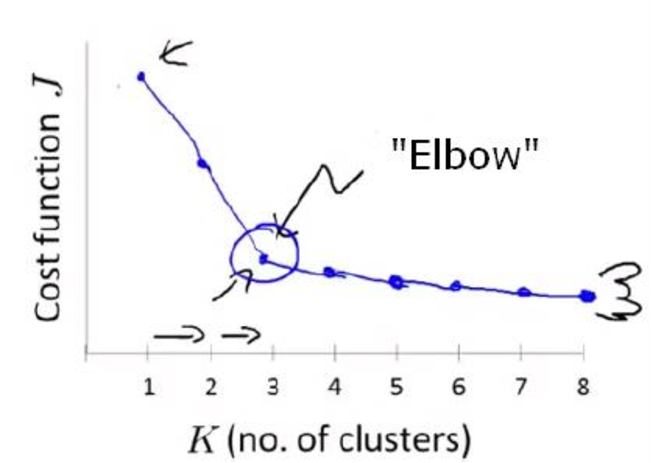
\includegraphics{TheorethicalFramework/dentification-of-Elbow-point.png}
  \caption{Illustration of determining $k$ using the "elbow" method \citep{kodinariya_review_2013}}
\end{figure}
In this situation, a Silhouette plot can be used to determine the $k$.
This method uses calculates the Silhouette coefficient for each cluster \citep{saputra_effect_2020}.
It takes into consideration the separation and cohesion of the cluster.
The plot can then be made by plotting the silhouette coefficient on the y-axis and $k$ on the x-axis \citep{saputra_effect_2020}.
Then the K with the highest coefficient can be selected based on that. \newline
Another popular method is the Gap statistic method \citep{yuan_research_2019}.
It compares the total within-cluster variation for different values of k with their expected values under a null reference distribution of the data \citep{tibshirani_estimating_2001}.
A practical appliance of this method uses a line plot for comparing the $k$-value and gap value \citep{yuan_research_2019}.
Based on the visual change of the line, someone is be-able to select the best $k$.

All in all, there is no fixed method to choose a good $k$ for K-means.
The elbow method is common in the existing literature and is very popular due to its simplicity.
However, one disadvantage is that it can be difficult to determine the "elbow" point, as it is not always present \citep{kodinariya_review_2013}.
In that case, the silhouette method or gap statistic method can be chosen, with the algorithm for silhouette being the most obvious choice due to its simplicity. \newpage
\subsubsection{Affinity Propagation} \label{theory:clustering-ap}
\gls{ap} is an algorithm that clusters data points by iteratively passing messages between them.
Each point sends and receives messages about the attractiveness of other points as cluster centers (exemplars) and the suitability of itself as a center \citep{keller_balancing_2021}.
The method was introduced by Frey et al. and does not require any hyperparameters \citep{frey_clustering_2007}.
Still, there are important properties that could potentially impact the clustering \citep{wang_adaptive_2007}. \newline
\textbf{Choosing preference($p$): }
Indicates the preference that a data point is selected as cluster center \citep{wang_adaptive_2007}.
It highly influences the number of clusters, a high one would lead to more clusters and a small one to less \citep{moiane_evaluation_2018}.
A good choice depending on the data is to set the $p$ to the median of all data similarities \citep{wang_adaptive_2007}.
But, the effectiveness of this could highly be influenced based on the dataset.
To validate if the preference is correctly set, it is possible to analyze the silhouette coefficient \citep{moiane_evaluation_2018}.
\newline
\textbf{Choosing damping factor($lam \in [0,1] $):}
The damping factor is used to improve the stability (convergence) of the algorithm \citep{wang_adaptive_2007}.
By default, this value is 0.5 and can be increased to 1 to reduce the impact of numerical oscillations.
This can be applied manually, by re-running the algorithm and finding the optimal or just being increased.
However, both approaches take a lot of time, especially for bigger datasets \citep{wang_adaptive_2007}. \newline

To conclude on this, damping is important if big datasets are considered.
However, this research does not use large datasets or consider time complexity as a metric.
The preference on the other hand could influence the results a lot.
For this, the silhouette coefficient can be evaluated to choose the best option.
In general, it should be sufficient to take the median.
\subsubsection{DBSCAN} \label{theory:clustering-dbscan}
\gls{dbscan} was introduced by \citep{ester_density-based_nodate} and works by drawing a radius (neighborhood) around data points.
It then groups all points within this radius as clusters. The main advantage is its ability to find arbitrarily shaped clusters and detect outliers \citep{liu_privacy_2012}.
To do this, the \gls{dbscan} algorithm uses the inputs $minPts$, $radius(\epsilon)$ and a distance function \citep{schubert_dbscan_2017}.
The $\epsilon$ is used to draw a neighborhood and the $minPts$ is used as a weight to evaluate which points should be inside the neighborhood.
For the distance function, the Euclidean distance is used, to be consistent with the other algorithms. \newline
\textbf{Choosing radius($\epsilon$):} The desired $\epsilon$ can be calculated using the K-NearestNeighbours algorithm \citep{ester_density-based_nodate,schubert_dbscan_2017}.
The general approach for this is to choose a $K = 2*N - 1$ (where N is the number of features) and plot the distance for each point.
This can then be plotted using a k-dist plot and the best "elbow" can be chosen for deciding the $\epsilon$ (similar to choosing the $k$ for K-means) \citep{elbatta_dynamic_2013}.
\begin{figure}[H]
  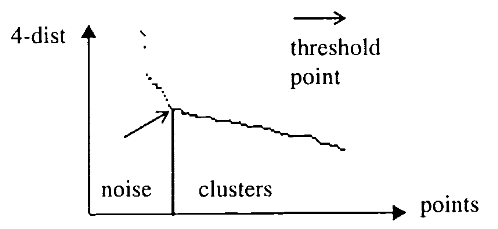
\includegraphics{TheorethicalFramework/K-dist-elbow.png}
  \caption{K-dist plot example for $minPts = 4$ based on a 2-dimensional dataset \citep{ester_density-based_nodate}}
  \label{k-dist-plot}
\end{figure}
\textbf{Choosing minimum points ($minPts$):} This hyperparameter is considered by a paper written by Sander et al.
The work describes a way of calculating this parameter by doing two times the feature amount \citep{sander_density-based_1998}.
So, using this approach a dataset with two features will have an $minPts$ of four.
This is confirmed by Schubert et al. to use the default $minPts = 4$ for a 2-dimensional dataset \citep{schubert_dbscan_2017}. \newline

In conclusion, the parameters of \gls{dbscan} are a little harder to estimate than for \gls{ap}.
But, as with K-means for $k$ there exists a selection method the $\epsilon$.
Although \gls{dbscan} requires the most hyperparameters out of the three clustering algorithms, determining them is clearer than for K-means.
There are clear methods for determining both the $minPts$ and $\epsilon$.

\subsubsection{Overfitting}

\subsection{Evaluation methods} \label{theory:evaluate}
Clustering comparison measures are important in cluster analysis for external validation by comparing clustering solutions to a "ground truth" clustering \citep{vinh_information_nodate-2}.
These external validity indices are a common way to assess the quality of unsupervised machine learning methods like clustering \citep{warrens_understanding_2022}.
A method that could be used for this is the Rand Index \citep{rand_objective_1971}.
It is a commonly applied method for comparing two different cluster algorithms \citep{wagner_comparing_nodate}.
An improvement of this method is adjusted for chance by considering the similarity of pairwise cluster comparisons \citep{vinh_information_nodate-2}.
Both the Rand Index (RI) and Adjusted Rand Index (ARI) \citep{hubert_comparing_1985-1} report a value between 0 and 1.
Where 0 is for no-similarity and 1 for identical clusters.
Alternatives for RI are the Fowles-Mallows Index and Mirkin Metric.
However, these two methods have their disadvantages. Respectively, being sensitive to a few clusters and cluster sizes \citep{wagner_comparing_nodate}.
The ARI metric suffers from cluster size imbalance as well, so it only provides not a lot of information on smaller clusters \citep{warrens_understanding_2022}.
Instead, they recommend using the cluster index metric that was proposed by Fränti et al. \citep{franti_centroid_2014}.

Another popular group of methods is the information theoric-based measures \citep{vinh_information_nodate-2}.
This metric measures the information between centroids; the higher the value, the better \citep{vinh_information_nodate-2}.
\gls{mi} is such metric, which calculates the probability of an element belonging to cluster $C$ or $C`$.
But, is not easy to interpret as it does not have a maximum value \citep{wagner_comparing_nodate}.
To this end, \gls{nmi} can be used to report a value between 0 and 1 using the geometric mean \citep{strehl_cluster_2002}.
The metric exists also in an adjusted version as \gls{ami}.
This works in the same way as for the \gls{ari} and is mostly needed if the number of data items is small in comparison to the number of clusters \citep{vinh_information_nodate-2}. \newline

Besides the external validity measurements for clustering, it is also possible to use internal validation methods.
These metrics focus entirely on the intrinsic dataset properties, instead of relying on an external baseline cluster algorithm \cite{craenendonck_using_nodate}.
Assessing two important concepts of clustering: compactness and separation \cite{hassani_using_2017}.
Both studies, consider three different metrics and measure both concepts at the same time \cite{hassani_using_2017}:
\begin{enumerate}
  \item \gls{chi} \citep{calinski_dendrite_1974-1} is used to measure the cluster variance (well-separated clusters) and low variance within the clusters (tightly coupled data). A high score indicates better clustering.
  \item Silhouette Index \citep{rousseeuw_silhouettes_1987} this metric is similar, by also measuring cohesion within clusters and separation of clusters. However, this metric uses the pairwise distance \cite{hassani_using_2017}. A score of -1 indicates incorrect clustering and +1 for dense clusters \cite{rousseeuw_silhouettes_1987}.
  \item Davies-Bouldin \citep{davies_cluster_1979} uses the average distance between centroids. A lower score indicates good clustering.
\end{enumerate}

K-Means scores relatively high for \gls{chi} \citep{craenendonck_using_nodate,hassani_using_2017} and SI \citep{craenendonck_using_nodate}.
The same applies to DBSCAN, which scores relatively high on SI and DB due to the sensitivity of noise \cite{craenendonck_using_nodate}.
% Thus, these metrics are difficult to use for very different cluster algorithms \cite{craenendonck_using_nodate}.
\subsubsection{Existing literature}
%A recent and much-cited study uses \gls{ari} and accuracy as metrics for evaluating K-Means \cite{ahmed_k-means_2020}.
%The accuracy is measured by calculating the percentage of the correct predicted labels and their truth labels.
Comparable studies with differential privacy use external validation \citep{xia_distributed_2020-1, sun_privbv_2022}.
Their experiment setup uses a so-called non-private cluster algorithm as external validation.
This cluster algorithm is trained without the perturbed data and compared with the same clustering algorithm that is trained with perturbed data.
Thus, the non-private variant functions as an external validation by providing the ground truth.

They compare the mutual information between a baseline cluster algorithm using \gls{ami} \citep{9679364} or \gls{nmi} \citep{xia_distributed_2020-1,sun_privbv_2022}.
Another study for evaluating \gls{dp} with \gls{ap} uses both \gls{ari} and \gls{ami}.
In addition to mutual information and rand index scores, it is also not uncommon to calculate the error between the two cluster algorithm's centroids \citep{xia_distributed_2020-1, 9679364}.
These two studies used Relative Error (RE) for this.